\chapter{The Berkeley Analog Generator}

\section{Overview and Top Level}
\begin{figure}[h]
\centering
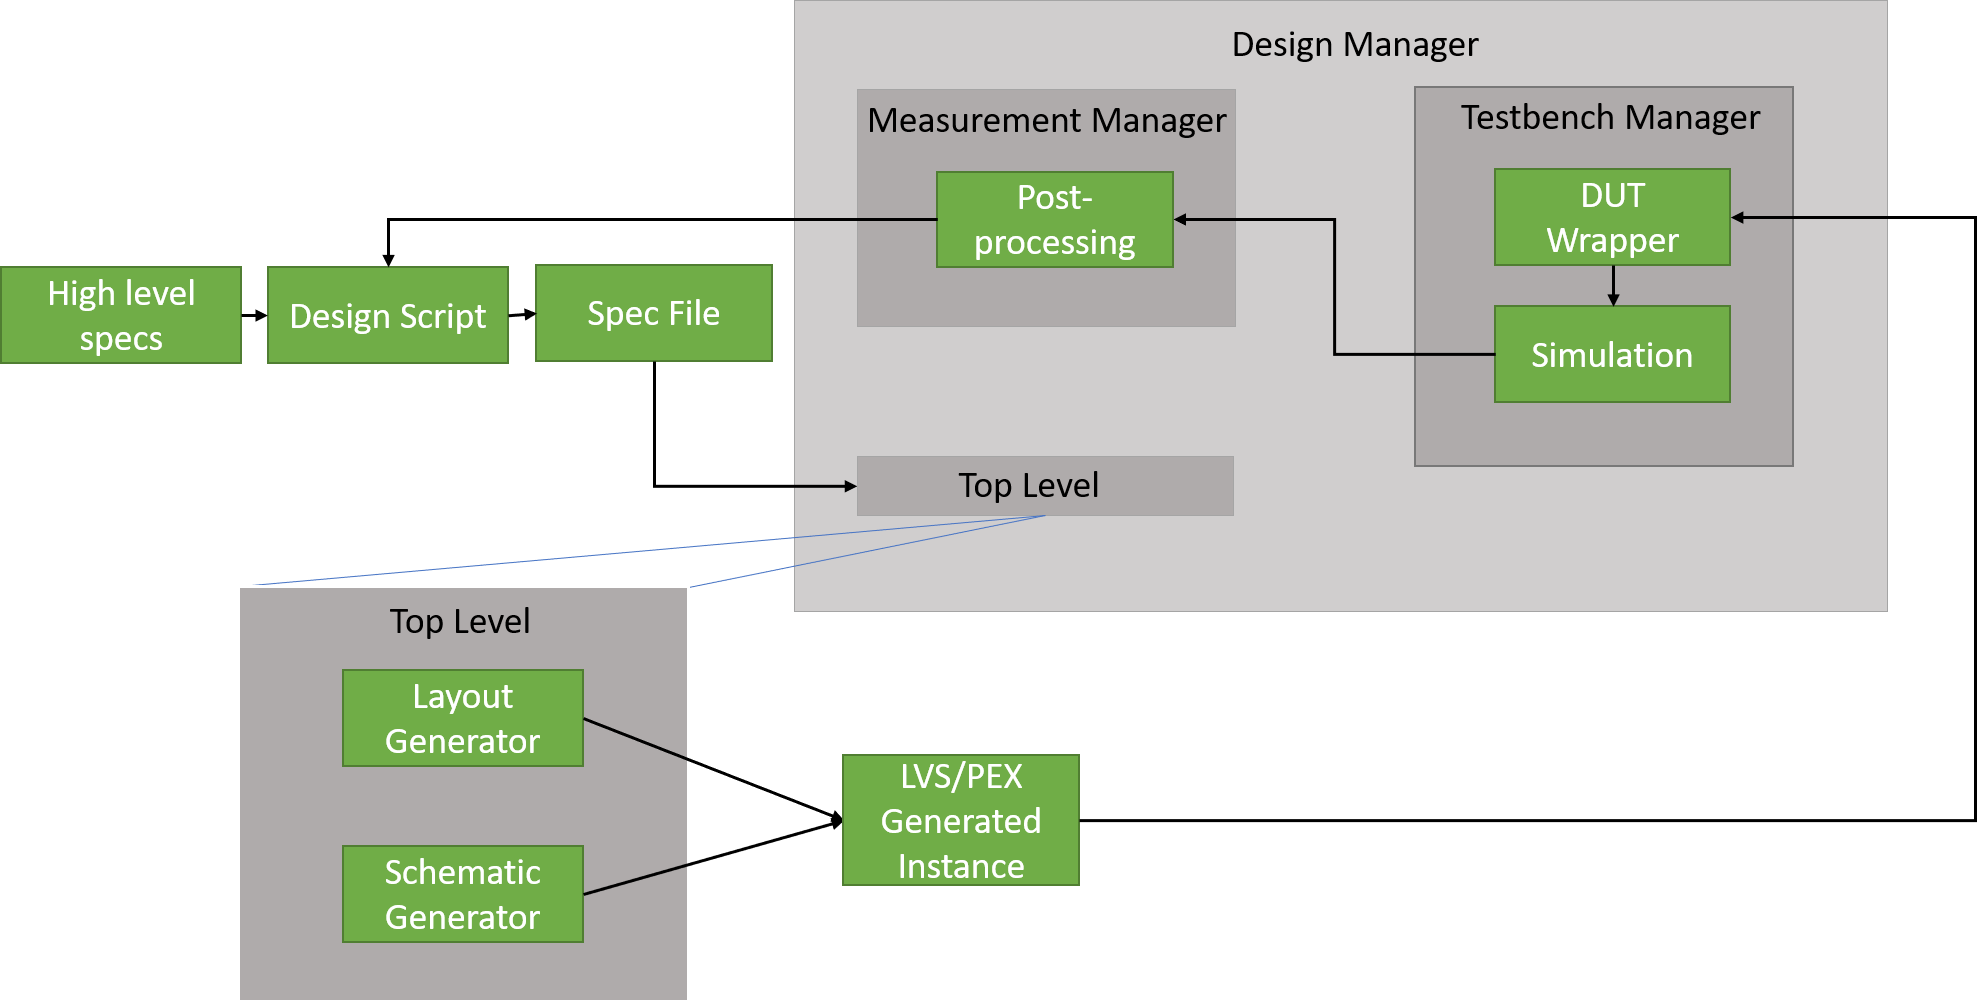
\includegraphics[width=0.8\textwidth]{bag_overview}
\caption{BAG Overview}
\label{fig:bag_top_level}
\end{figure}
As discussed in \cite{chang_bag2:_2018}, BAG is a framework that allows users to create, use and test process-portable analog generators. Designers can create template schematics and write a scripted layout generator that incorporates their design methodology in a technology agnostic, parametrized way. At the highest level, the user inputs parameters, examples of which will be shown later in this chapter and in Chapter 3, such as device dimensions and passive component values into a specification file, and a script will generate a schematic, LVS tested layout and a PEX netlist. The main advantage is that the delay of the design loop discussed in Chapter 1 is significantly reduced as post-layout effects can be directly included into the flow. 

As will be discussed in later sections, there are a few main components to a ``complete" generator. At the lowest levels are the layout generator and schematic generator. These are responsible for the physical process of generating the circuit representation and layout. In order to use these, there is also a top level script that reads a parameter file and runs the schematic/layout generators with these specifications. The top level is also responsible for deciding whether or not to run LVS/PEX on the generated instance.

At an even higher level is the notion of a design script and design managers. Design manager is a class responsible for using the top level generator mentioned previously and overseeing the process of running tests and post-processing on test results. Design manager has associated test bench scripts which are responsible for connecting the generated device into a previously made test harness. The test bench script maps the pins of the instance to the pins of the test harness and runs predetermined SPICE simulations (i.e. AC, transient, S-parameters) before exporting the results to Python. Design manager can then pass the results to a measurement manager which can process, plot, etc. The entire process can be visualized as in Figure \ref{fig:bag_top_level}.

The notion of a design script is an even higher level concept which allows a designer to encode their design procedure automatically into a close-looped script. The user can write a script that computes passive and transistor sizings, allow design manager to generate and test the post-PEX netlist, and iterate based on the results. The possibility of incorporating a design script will be discussed later, although a design script is not presented in this work. Design scripts are discussed in further detail in \cite{chang_bag2:_2018} and \cite{hakhamaneshi_late_nodate}.

\section{Layout Generators}
Layout generators are arguably the most important portion of the process and are extensively discussed in \cite{chang_bag2:_2018}. BAG offers a set of functions for drawing transistors, automatically routing metals, drawing vias, etc. to allow the same capability that hand design would produce. The goal of the designer is to use these functions in a generic way that automatically computes where and how to draw connections that will be DRC and LVS clean regardless of the input specifications. 

The typical process of generating a large complex block is to start with small cells, like an inverter or an active diff amp using \texttt{AnalogBase}. \texttt{AnalogBase} is a class in BAG used for drawing layouts comprised entirely of transistors. Firstly, the user draws a schematic template, like shown in Figure \ref{fig:sch_templ}.
\begin{figure}[h]
\centering
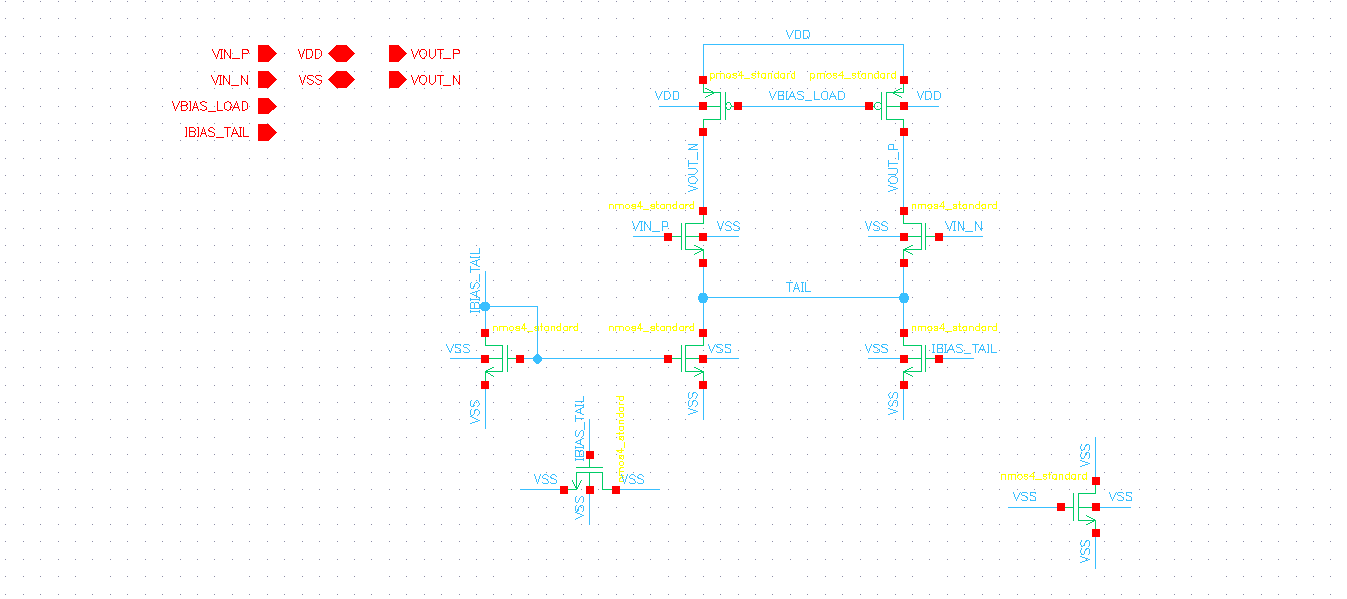
\includegraphics[width=0.8\textwidth]{sch_temp}
\caption{Differential amplifier schematic template example}
\label{fig:sch_templ}
\end{figure}
\clearpage
This template holds only a human-readable description of the connections. The schematic will be copied over with actual values filled in by BAG afterward. One thing to note is the presence of seemingly useless transistors, like in the bottom right. These transistors are used by BAG to properly create dummy transistors in the layout, and anything else can be removed if not used in the schematic generator. Additionally, the transistor in the bottom left used for adding stabilization capacitance can also be removed if desired. Example layouts below will not have this transistor.

Using the schematic template, the user then decides how many rows of transistors will be in the layout, and assigns a number of transistors to each row. There are a number of helper functions to generate a data structure containing information about which row the transistor is in, the drain/source metal directions, number of fingers, etc. which is called the ``initialization step". An example of how one might set up the rows and initialization for the amplifier in Figure \ref{fig:sch_templ} is shown in Listing \ref{lst:rows_assign} and Listing \ref{lst:tx_init}. Note that these code blocks are only portions of the full layout generator and there are, in general, a small number of extra lines required. This section highlights only the most important portions of a generator.
\begin{lstlisting}[language=Python, caption=Creating rows for transistors, label={lst:rows_assign}, float]
        # Rows are ordered from bottom to top
        # To use TrackManager, an ordered list of wiring types and their locations must be provided.
        # Define two lists, one for the nch rows and one for the pch rows
        # The lists are composed of dictionaries, one per row.
        # Each dictionary has two list entries (g and ds), which are ordered lists of what wire types will be present
        #  in the g and ds sections of that row. Ordering is from bottom to top of the design.
        wire_names = dict(
            nch=[
                # tail row
                dict(
                    g=['bias'],
                    ds=['bias']
                ),
                # Input row
                dict(
                    g=['sig'],
                    ds=['sig']
                )
            ],
            pch=[
                # top row
                dict(
                    ds=['sig'],
                    g=['bias']
                )
            ]
        )
        layout_helper.wire_names = wire_names
        # Set up the row information
        # Row information contains the row properties like width/number of fins, orientation, intent, etc.
        # Storing in a row dictionary/object allows for convenient fetching of data in later functions
        row_tail = layout_helper.initialize_rows(row_name='tail',
                                        orient='R0',
                                        nch_or_pch='nch',
                                        )
        row_input = layout_helper.initialize_rows(row_name='input',
                                         orient='R0',
                                         nch_or_pch='nch',
                                         )
        row_mirror = layout_helper.initialize_rows(row_name='top',
                                          orient='R0',
                                          nch_or_pch='pch',
                                          )

        # Define the order of the rows (bottom to top) for this analogBase cell
        layout_helper.global_rows = [row_tail, row_input, row_mirror]
\end{lstlisting}
\clearpage
\begin{lstlisting}[language=Python, caption=Assigning transistors to a row and initializing, label={lst:tx_init}, float]
	      ################################################################################
        # 2:
        # Initialize the transistors in the design
        # Storing each transistor's information (name, location, row, size, etc) in a 
        # dictionary object allows for convenient use later in the code, and also
        # greatly simplifies the schematic generation
        # The initialization sets the transistor's row, width, and source/drain net names
        # for proper dummy creation
        ################################################################################
        tail_l = layout_helper.initialize_tx(name='tail_l', row=row_tail,
                     fg_spec='bottom_tail',
                     deff_net='TAIL')
        tail_r = layout_helper.initialize_tx(name='tail_r', row=row_tail,
                     fg_spec='bottom_tail',
                     deff_net='TAIL')
        bias = layout_helper.initialize_tx(name='bias', row=row_tail,
                     fg_spec='bottom_bias',
                     deff_net='IBIAS_TAIL')
        in_left = layout_helper.initialize_tx(name='in_left', row=row_input,
                     fg_spec='bottom_in',
                     seff_net='TAIL', deff_net='VOUT_N')
        in_right = layout_helper.initialize_tx(name='in_right', row=row_input,
                     fg_spec='bottom_in',
                     seff_net='TAIL', deff_net='VOUT_P')
        top_left = layout_helper.initialize_tx(name='top_left', row=row_mirror,
                     fg_spec='top',
                     deff_net='VOUT_N')
        top_right = layout_helper.initialize_tx(name='top_right', row=row_mirror,
                     fg_spec='top',
                     deff_net='VOUT_P')
\end{lstlisting}
\clearpage
\begin{lstlisting}[language=Python, caption=Assigning transistors to columns, label={lst:col_assign}, float]
	      # Calculate positions of transistors
        # This uses helper functions to place each transistor within a stack/column of a
        # specified starting index and
        # width, and with a certain alignment (left, right, centered) within that column
        layout_helper.assign_tx_column(tx=bias, offset=col_mid, fg_col=fg_mid, align=0)
        layout_helper.assign_tx_column(tx=tail_l, offset=col_stack_left, 
           fg_col=fg_stack, align=0)
        layout_helper.assign_tx_column(tx=in_left, offset=col_stack_left,
           fg_col=fg_stack, align=0)
        layout_helper.assign_tx_column(tx=top_left, offset=col_stack_left, 
           fg_col=fg_stack, align=0)
        layout_helper.assign_tx_column(tx=tail_r, offset=col_stack_right, 
           fg_col=fg_stack, align=0)
        layout_helper.assign_tx_column(tx=in_right, offset=col_stack_right,
           fg_col=fg_stack, align=0)
        layout_helper.assign_tx_column(tx=top_right, offset=col_stack_right, 
           fg_col=fg_stack, align=0)
\end{lstlisting}
After initializing all transistors, the user then must specify their locations in the layout by creating fictitious columns that stacks of transistors will be placed in. Based on the number of fingers each transistor has, technology required spacing and any other spacing (to route dummies, etc.) the user can compute columns based on a number of fingers, and assign the transistors like in Listing \ref{lst:col_assign}.

The final transistor placement step is to set the drain and source orientations. A transistor's source can be routed up or down which affects where the gate placements are made, and the first diffusion region per transistor can be either source or drain to make alignment simpler. There is also a helper function to automatically compute based on number of fingers which region should be the source or drain based on another transistor the user wishes to align to. This is shown in Listing \ref{lst:sd_align}.
\begin{lstlisting}[language=Python, caption=Determining transistor drain/source configurations, label={lst:sd_align}, float]
	      ################################################################################
        # 4:  Assign the transistor directions (s/d up vs down)
        #
        # Specify the directions that connections to the source and connections to the drain
        # will go (up vs down). Doing so will also determine how the gate is aligned
        # (ie will it be aligned to the source or drain)
        # See the bootcamp for more details
        # The helper functions used here help to abstract away whether the intended 
        # source/drain diffusion region of a transistor occurs on the even or odd
        # columns of that device (BAG always considers the even columns of a 
        # device to be the 's'). These helper functions allow a user to specify 
        # whether the even columns should be the transistors effective source or
        # effective drain, so that the user does not need to worry about BAG's notation.
        ################################################################################

        # Set tail bias tx  to have source on the leftmost diffusion (arbitrary)
        # and source going down
        layout_helper.set_tx_directions(tx=bias, seff='d', seff_dir=0)
        # Assign the input to be anti-aligned, so that the input source and tail
        # drain are vertically aligned
        layout_helper.set_tx_directions(tx=in_left, seff='s', seff_dir=0)
        layout_helper.set_tx_directions(tx=in_right, seff='s', seff_dir=0)

        layout_helper.assign_tx_matched_direction(target_tx=tail_l, source_tx=in_left,
             seff_dir=0, aligned=False)
        layout_helper.assign_tx_matched_direction(target_tx=tail_r, source_tx=in_right,
             seff_dir=0, aligned=False)

        layout_helper.assign_tx_matched_direction(target_tx=top_left, 
             source_tx=in_left, seff_dir=2)
        layout_helper.assign_tx_matched_direction(target_tx=top_right, 
             source_tx=in_right, seff_dir=2)
\end{lstlisting}
\clearpage
Finally, the difficult setup is complete, and the user can call the function \texttt{self.draw\_base()} with the information about rows, transistors, etc. set up in the previous steps. BAG will then draw the all of the required polygons for the metal connections to the MOS devices and everything else. An example base layout with no wiring done of the schematic in Figure \ref{fig:sch_templ} is shown in Figure \ref{fig:base_layout_metal}.
\begin{figure}[h]
\centering
\begin{subfigure}{.4\linewidth}
  \centering
  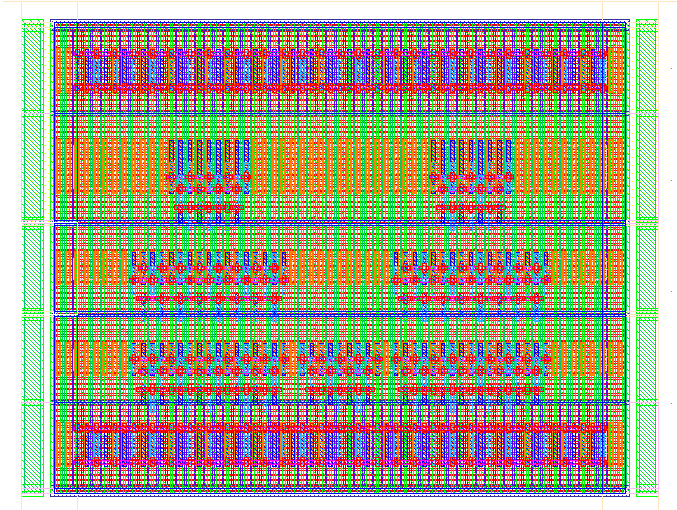
\includegraphics[width=\textwidth]{base_full}
  \caption{Base layout of transistors with active regions, poly, etc.}
  \label{fig:sfig1}
\end{subfigure}
\begin{subfigure}{.4\linewidth}
  \centering
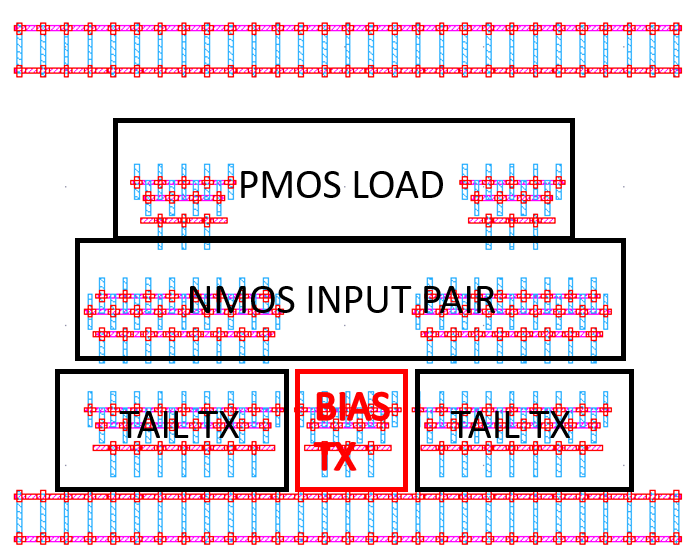
\includegraphics[width=0.9\textwidth]{base_metal_annotated}
  \caption{The same layout with only metal connection layers shown. Annotated with locations of transistors.}
  \label{fig:sfig2}
\end{subfigure}
\caption{Base layout}
\label{fig:base_layout_metal}
\end{figure}
\clearpage
After drawing the base layout, users can then specify how to connect wires and ports by specifying a metal layer, a wire width and a track. Tracks are an invisible grid that spans the design space used by BAG to place wires properly. Listing \ref{lst:wiring} shows an example command of how to connect elements. Note that this code makes no reference to anything specific nor does it ``hardcode" any parameters. Everything is generic to the specified parameters. Figure \ref{fig:base_with_wires} shows the connections made by BAG.
\begin{lstlisting}[language=Python, caption=Drawing wire connections., label={lst:wiring}, float]
	      #Connect up bias gates + drain
        warr_bias_in = self.connect_to_tracks(
            [tail_l['g'], tail_r['g'], bias['d'], bias['g']],
            tid_tail_gate
        )
        #connect tail drains to input sources (tail node)
        warr_tail = self.connect_to_tracks(
            [tail_l['d'], tail_r['d'], in_right['s'], in_left['s']],
            tid_tail_ds
        )
\end{lstlisting}
\begin{figure}[h]
\centering
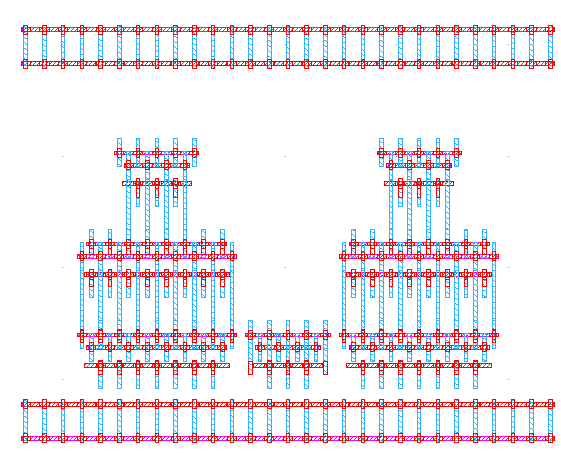
\includegraphics[width=0.6\textwidth]{base_metal_conns}
\caption{Transistor wiring}
\label{fig:base_with_wires}
\end{figure}

Lastly, the user finalizes connections and adds pins to wires. In the final step, BAG will draw dummy transistors and create straps for the power supplies, automatically routing the dummies' connections to the supply, like in Figure \ref{fig:finished_layout}.
\begin{figure}[h]
\centering
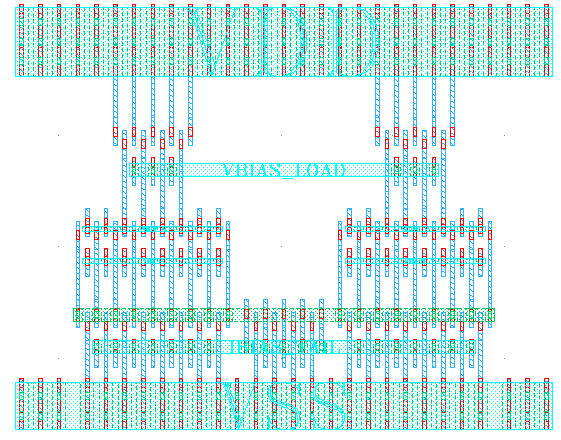
\includegraphics[width=0.6\textwidth]{full_layout}
\caption{Finished layout (only metals shown)}
\label{fig:finished_layout}
\end{figure}
With a finished layout generator, the user can now arbitrarily change their transistor specifications which will be reflected automatically in the wiring and sizing. Figure \ref{fig:width_changes} shows the same generator with various width and number of finger choices. An important note is that the user can do all this without knowing any of the myriad of the layout design rules since BAG handles these complexities internally and abstracts them away from the user.
\begin{figure}[h]
\centering
\begin{subfigure}{.4\linewidth}
  \centering
  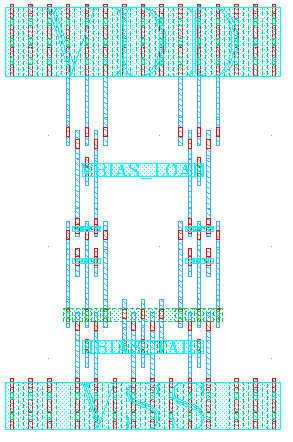
\includegraphics[width=0.6\textwidth]{small_width}
  \caption{}
  \label{fig:sfig1}
\end{subfigure}
\begin{subfigure}{.4\linewidth}
  \centering
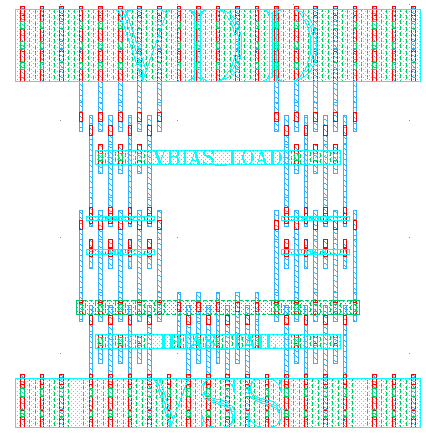
\includegraphics[width=0.6\textwidth]{med_width}
  \caption{}
  \label{fig:sfig2}
\end{subfigure}
\begin{subfigure}{.4\linewidth}
  \centering
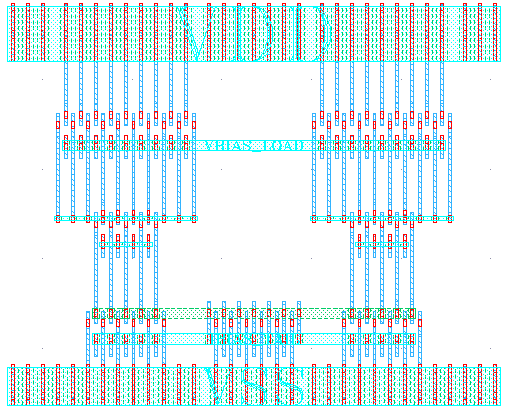
\includegraphics[width=0.6\textwidth]{large_width}
  \caption{}
  \label{fig:sfig2}
\end{subfigure}
\caption{Differential amplifier layout with various widths and number of finger choices.}
\label{fig:width_changes}
\end{figure}
\clearpage
BAG also offers hierarchy in layout using \texttt{TemplateBase} \cite{chang_bag2:_2018}. When a library of smaller cells are created, the user can then ``stamp" these cells into a larger unit and connect them together to form more complex systems. Listing \ref{lst:master_creation} demonstrates the code to insert a double tail sense amplifier into a circuit. The user first creates a template, then computes a location where the circuit should be placed using helper functions to guarentee everything is aligned to the grid. Lastly, with the computed coordinates, the user can instantiate the circuit into the layout. An example of a circuit containing a differential transimpedance amplifier (TIA) and continuous-time linear equalizer (CTLE) is shown in Figure \ref{fig:tia_ctle}.
\begin{lstlisting}[language=Python, caption=Adding and placing templates to a layout, label={lst:master_creation}, float]
# Define the instance masters
	...
        master_dtsa = self.new_template(params=dtsa_params, 
            temp_cls=DoubleTailSenseAmplifier)
	...
	...
	...
	      x, y = layout_helper.get_on_track_offset(
            master_dtsa,
            x_offset=largest/2 + master_dtsa.bound_box.right_unit/2,
            y_offset=wiring_space + inst_combined.bound_box.top_unit,
            unit_mode=True
        )

        inst_dtsa = self.add_instance(
            master_dtsa, 'XDTSA',
            loc=(x, y),
            orient='MY',
            unit_mode=True
        )
\end{lstlisting}
\begin{figure}[h]
\centering
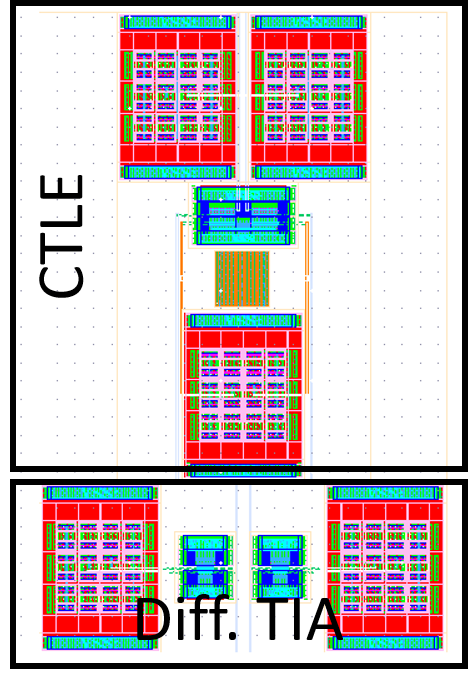
\includegraphics[width=0.4\textwidth]{tia_ctle_annotated}
\caption{Differential TIA and CTLE}
\label{fig:tia_ctle}
\end{figure}

The benefit of codifying the layout procedure is that configuration can be automatically included. For example, should a designer want variable resistors in their circuit, they may opt for a resistor DAC. Resistor DACs are often an arbitrary number of arrayed unit resistors with digitally controlled switches. One method of implementing such a resistor DAC is a set of series resistors each with a parallel switch that can short out or connect any of the series resistors. Using \texttt{TemplateBase}, we can place any amount of template layouts which allows for a single generator with a large degree of freedom to create such a circuit. The user can choose how many bits, what type of switch to use (NMOS, PMOS, passgate), and even whether or not to include local inversion for the passgate. An example of multiple resistor DAC layouts of this style are shown in Figure \ref{fig:dac} and a small portion of the configuration file in Listing \ref{lst:res_dac_params}.
\begin{lstlisting}[language=Python, caption=Resistor DAC params sample, label={lst:res_dac_params}, float]
params:
  output_bits_dir: 'left' #where to drag the control bits to
  bits: 1
  switch_params:
    switch_type: 'transmission'
    include_inv: True
    switch_params:
      lch: !!float 14e-9
      guard_ring_nf: 0
      ptap_w: 6
      ntap_w: 6
      w_dict:  # Width of each row. Each row needs the width specified
        nmos:  6
        pmos:  12

      th_dict:  # Threshold information / thick ox / etc for each row
        nmos: 'standard'
        pmos: 'standard'

      seg_dict:  # Number of fingers of each transistor
        nmos: 8
        pmos: 16
...
...
...
res_params:
    show_pins: True
    l: 0.5e-6
    w: 1.0e-6
    sub_type: 'ptap'
    threshold: 'standard'
    nser: 1
    npar: 1
    ndum: 1
    port_layer: 5
...
...
...
\end{lstlisting}
\clearpage
\begin{figure}[h]
\centering
\begin{subfigure}{1\linewidth}
  \centering
  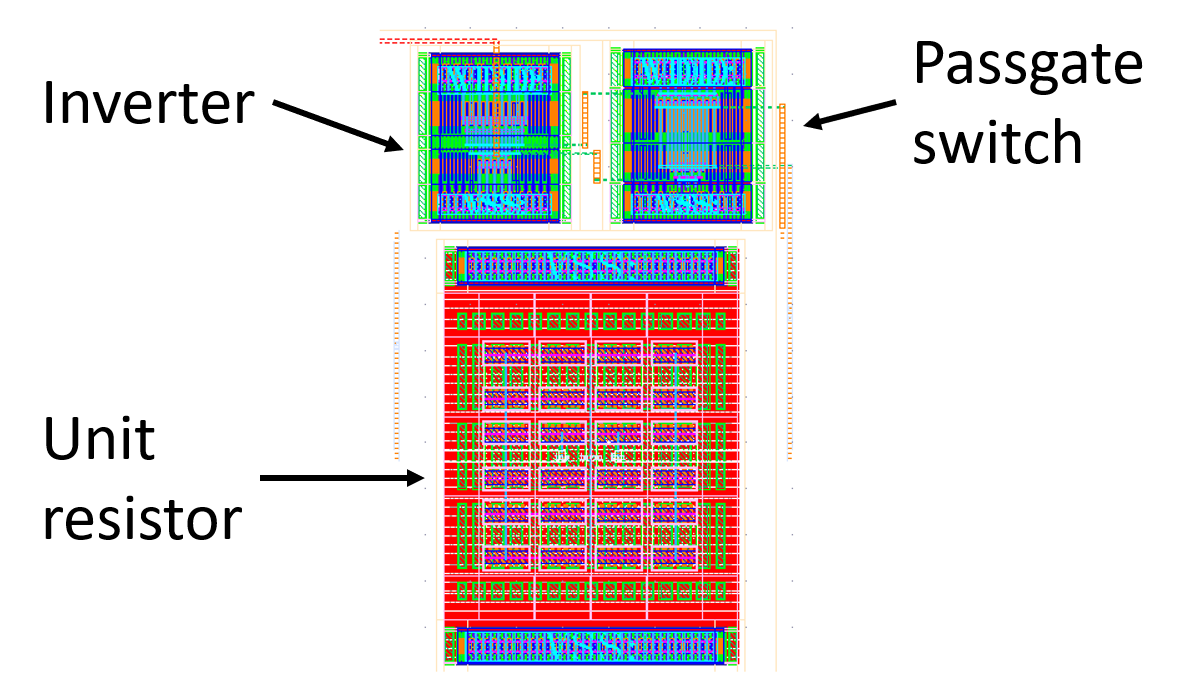
\includegraphics[width=0.4\textwidth]{res_dac_1_annotated}
  \caption{1 bit}
  \label{fig:sfig1}
\end{subfigure}
\begin{subfigure}{.4\linewidth}
  \centering
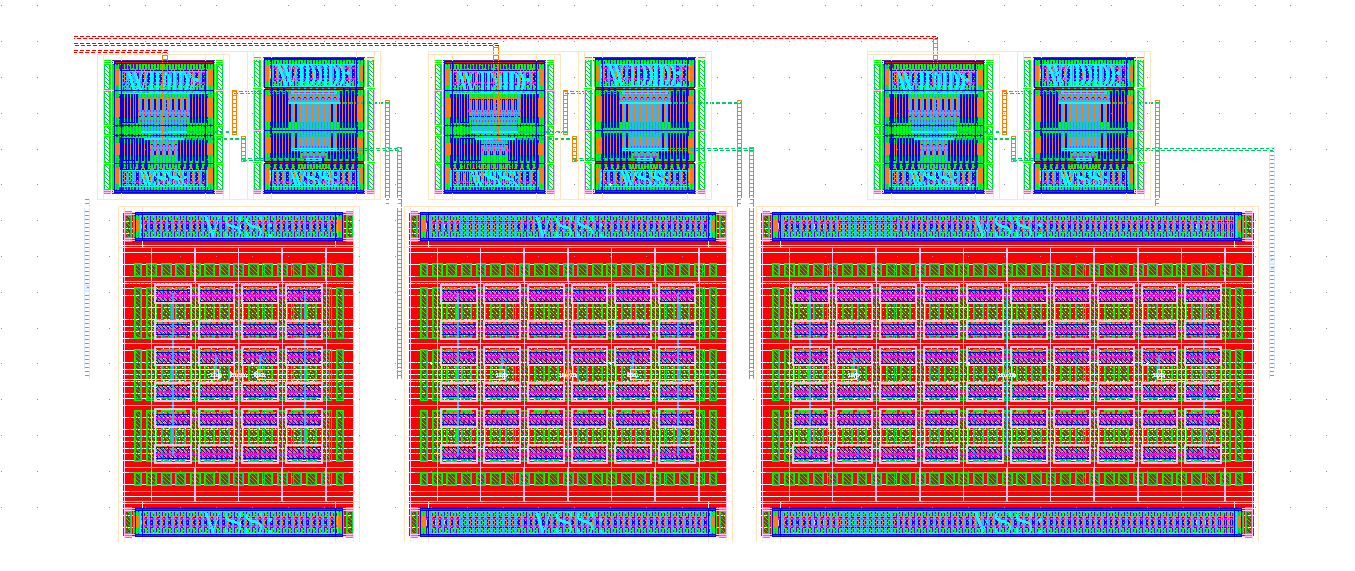
\includegraphics[width=1\textwidth]{res_dac_3}
  \caption{3 bits}
  \label{fig:sfig2}
\end{subfigure}
\begin{subfigure}{.5\linewidth}
  \centering
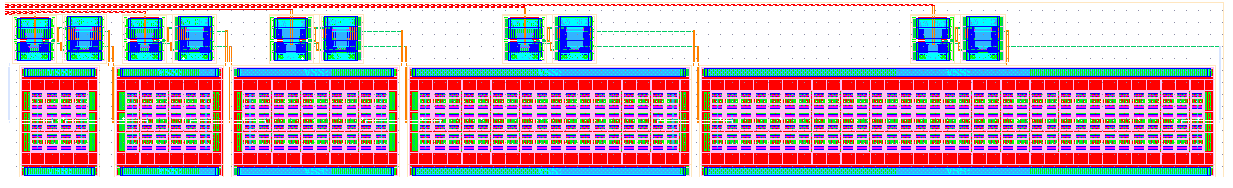
\includegraphics[width=1.2\textwidth]{res_dac_5}
  \caption{5 bits}
  \label{fig:sfig2}
\end{subfigure}
\caption{Various resistor DAC generated layouts}
\label{fig:dac}
\end{figure}
\clearpage
\section{Schematic Generators}
Schematic generators control the process of copying the template schematic mentioned previously and assigning values to the components based on the inputted spec file \cite{chang_bag2:_2018}. These generators have the capability of arraying and deleting instances, removing, adding or renaming pins and other simple operations.

Generally the user simply inputs commands to pass the component values into the design; but for circuits such as the resistor DAC in the previous section, the user can automatically array and resize components based on the layout like shown in Figure \ref{fig:resdac_sch}. Portions of the code that accomplishes this is shown in Listing \ref{lst:res_dac_sch_code}.
\begin{lstlisting}[language=Python, caption=Resistor DAC schematic generator, label={lst:res_dac_sch_code}, float]
# Some pins are not needed depending on the type of switch used.
if switch_type == 'nmos':
        self.remove_pin('CTRL_B')
        self.remove_pin('VDD')
    else:
        if include_inv:
            self.remove_pin('CTRL_B')
        else:
            if switch_type == 'pmos':
                self.remove_pin('CTRL')
# When using a multi-bit resDAC, rename the input pin to have the required bitwidth.
    if bits > 1:
        if switch_type == 'nmos':
            self.rename_pin('CTRL', 'CTRL<' + str(bits-1) + ":0>")
        else:
            if include_inv or switch_type == 'transmission':
                self.rename_pin('CTRL', 'CTRL<' + str(bits - 1) + ":0>")
            if not include_inv:
                self.rename_pin('CTRL_B', 'CTRL_B<' + str(bits-1) + ":0>")
...
...
...
# Copy the unit cell many times with many names
self.array_instance('X_SWITCH0', switch_names, switch_port_names)
self.array_instance('X_RES0', res_names, res_port_names)
...
...
...
#Loop through all instances and use the design method to input the params from the spec file into the schematic
for ind, inst in enumerate(self.instances['X_RES0']):
	inst.design(**res_params_list[ind])
\end{lstlisting}
\clearpage
\begin{figure}[h]
\centering
\begin{subfigure}{.5\linewidth}
  \centering
  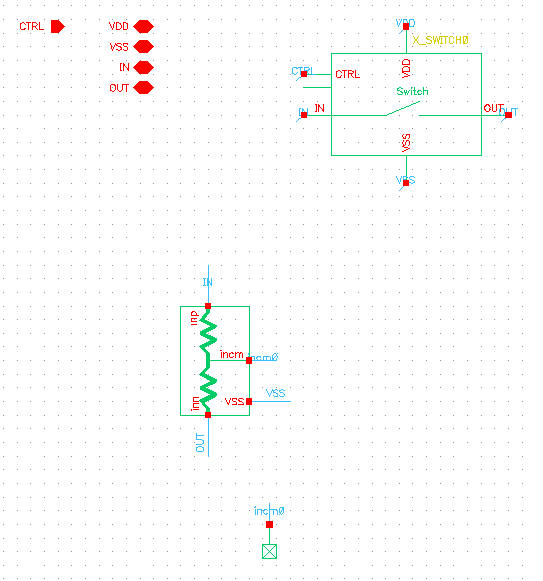
\includegraphics[width=\textwidth]{res_dac_1_sch}
  \caption{1 bit}
  \label{fig:sfig1}
\end{subfigure}
\begin{subfigure}{0.6\linewidth}
  \centering
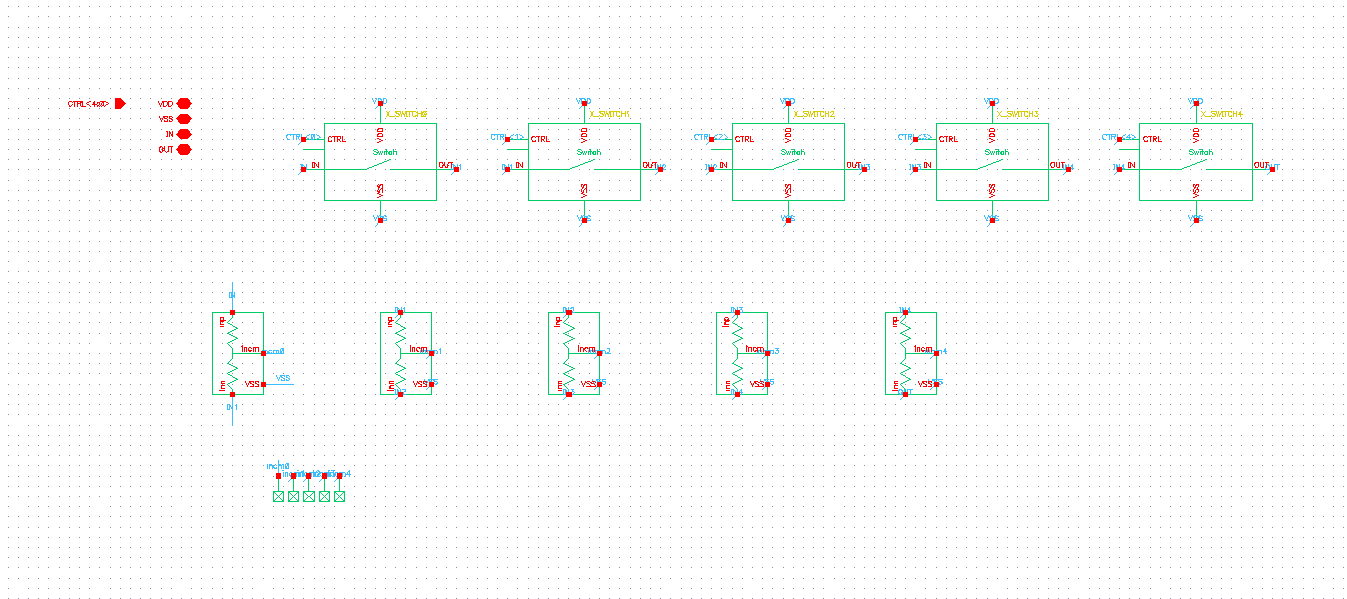
\includegraphics[width=\textwidth]{res_dac_5_sch}
  \caption{5 bits}
  \label{fig:sfig2}
\end{subfigure}
\caption{Various resistor DAC schematics}
\label{fig:resdac_sch}
\end{figure}
\clearpage
\section{Design Manager and Test Benches}
As shown in Figure \ref{fig:bag_top_level}, design manager is a higher level entity to that of the layout and schematic generators \cite{chang_bag2:_2018}. Design managers contain within them multiple test bench managers that each have their own corresponding measurement manager. In the specifications file, the user decides which tests to run and design manager will generate an instance and pass it through the chosen simulations. This is the method used to test the circuits described in Chapter 4. 

Tests are made by the user in a similar method to schematic generators. The user specifies a test bench setup with a generic DUT block and adds input sources and pins. Within a specifications file, the user describes how to wrap the inputs of the DUT to the generic block, as well as what outputs to save. These outputs are sent to the measurement manager where the user can, for example, compute 3dB frequencies, DC gain, etc. and save the results if desired. Multiple test benches can be run in one instance. A portion of an example parameters file for testbench management is shown in Listing \ref{lst:tb_manager_yaml}.
\begin{lstlisting}[language=Python, caption=Test bench parameters, label={lst:tb_manager_yaml}, float]
#Specifying how the ports of the device map to the generic DUT template
dut_wrappers:
  - name: 'ac_forward'
    lib: 'bag_testbenches_kh'
    cell: 'diff2SingleEnded_wrapper_ac_forward'
    params:
      dut_conns:
        IBIAS_TAIL: 'IBIAS_TAIL'
        VIN_N: 'VIN'
        VIN_P: 'VIP'
        VSS: 'VSS'
        VDD: 'VDD'
        VOUT_N: 'VON'
        VOUT_P: 'VOP'
#Choosing which measurement classes to run
measurements:
    #The - next to meas_type is not a mistake. It specifies that the entire contents of measurements is a list.
  - meas_type: 'CTLE_char'
    meas_package: 'verification_kh.CTLEMeasurementUnit'
    meas_class: 'CTLEMeasurementManager'
    out_fname: 'CTLE_char.yaml'
    sch_params: {}
    testbenches:
        ac_forward:
          tb_package: 'verification_kh.GenericACTB'
          tb_class: 'GenericACTB'
          tb_lib: 'bag_testbenches_ec'
          tb_cell: 'amp_tb_ac'
          wrapper_type: 'ac_forward'

    ...
	  ...
	  ...

	  #Specify simulation variables
          fstart: !!float 1e3
          fstop: !!float 10e10
          fndec: 10
          sim_vars:
            ibias: !!float 900e-06
            vdd: !!float 0.8
            cload: !!float 20.0e-15
            vicm: !!float 0.6
	  #Choose what outputs to save
          sim_outputs:
            outdiff: "VF(\"/vout\")"
            outcm: "VF(\"/vout_cm\")"
            indiff: "VF(\"/vin\")"
            ibias: "IDC(\"/VSUP/PLUS\")"
\end{lstlisting}
\clearpage
An example test bench manager, \texttt{generic\_AC\_TB},\footnote{This test bench, and all others used in this report come courtesy of Kourosh H. of team Vlada.} inputs an AC voltage or current and runs an AC simulation and noise simulation. The corresponding measurement manager sifts through the data and (regardless of the transfer function shape) computes the DC gain and overall bandwidth. The noise data is integrated and reported, as well as CMRR. 

Since BAG is written in Python, users can easily extend or add features to BAG. An example is the extension of \texttt{DesignManager} to \texttt{SweepDesignManager}. This subclass inherits all the basic properties and functions in design manager, but allows the user to specify a set of variables in the parameter file to sweep. BAG will then automatically generate one instance per parameter value in the range, and simulate them all in parallel. This allows for the same type of sweeps one would do manually, but additionally includes parasitics and LVS.